%!TEX root = ../../../super_main.tex

\section{Collaboration with Group \emph{SW613F15}}
\label{sec:collaboration_with_group_sw613f15}

\todo{HOOOHOHOHOHOHOLM START}
After the recent handover of \gc from group our group to \emph{SW613F15}, it was discovered that a component in \ps was not consistent with the design implemented in the \launcher regarding showing of multiple items, applications and pictograms respectively. This inconsistency can be seen in \figref{fig:collab_with_group_13}.
\todo{HOOOHOHOHOHOHOLM END}

\begin{figure}[!htbp]
    \centering

    \begin{subfigure}[t]{0.75\textwidth}
        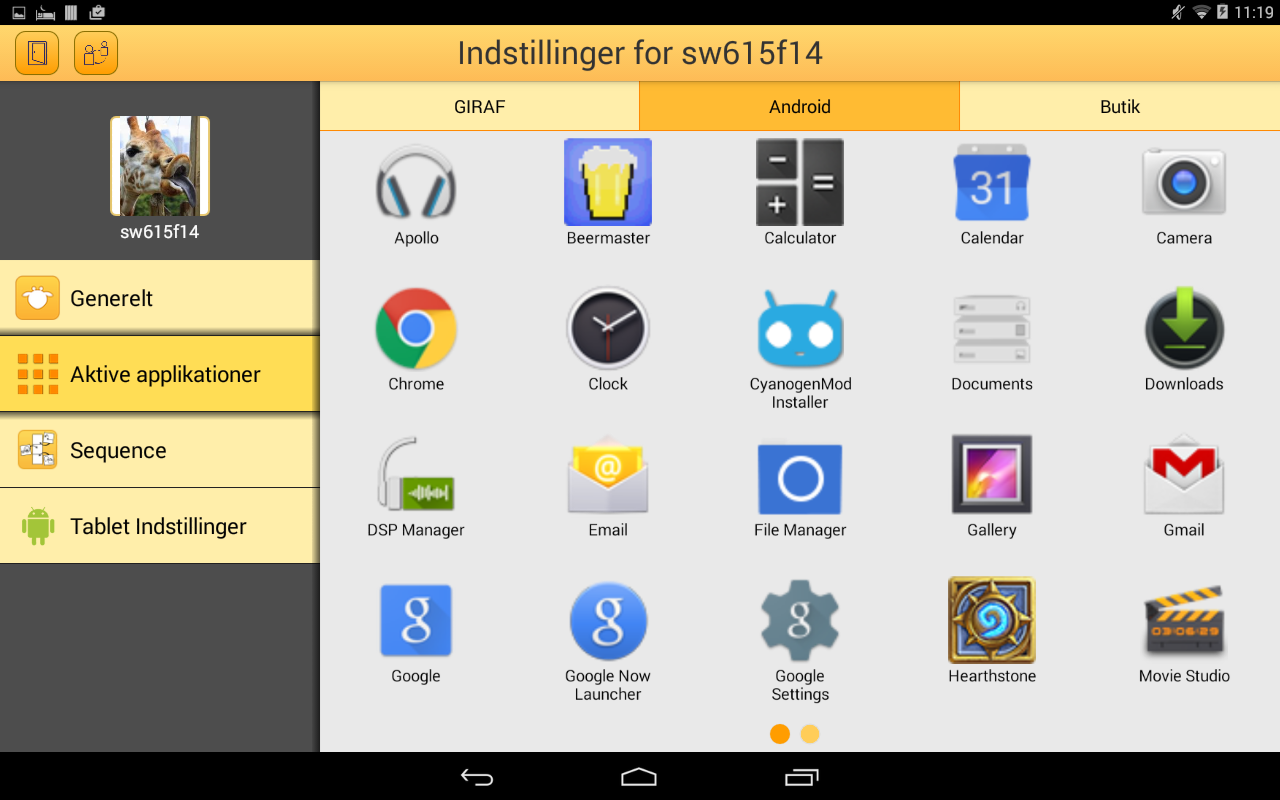
\includegraphics[width=\textwidth]{sprint_three/collab_with_group_13/launcher.png}
        \caption{The \launcher application}
        \label{fig:collab_with_group_13_launhcer}
        \vspace*{1cm}
    \end{subfigure}
    \hfill
    \begin{subfigure}[t]{0.75\textwidth}
        \includegraphics[width=\textwidth]{sprint_three/collab_with_group_13/pictosearch.png}
        \caption{The old \ps application}
        \label{fig:collab_with_group_13_pictosearch}
    \end{subfigure}
    
    \caption{Problem visualized}
    \label{fig:collab_with_group_13}
\end{figure}

Our group had already spent some time on implementing a \androidinline{ViewPager} for the \launcher (see \secref{sec:reengineering_of_application_grid}). For this reason, a solution for \ps was made in collaboration with group \emph{SW613F15}. A slight implementation difference was that the \androidinline{ViewPager} in the launcher is implemented using fragments, whereas the \androidinline{ViewPager} in \ps is implemented using views. This solution can be seen in \figref{fig:pictosearch_view_pager}. 

\begin{figure}[!htbp]
    \centering
    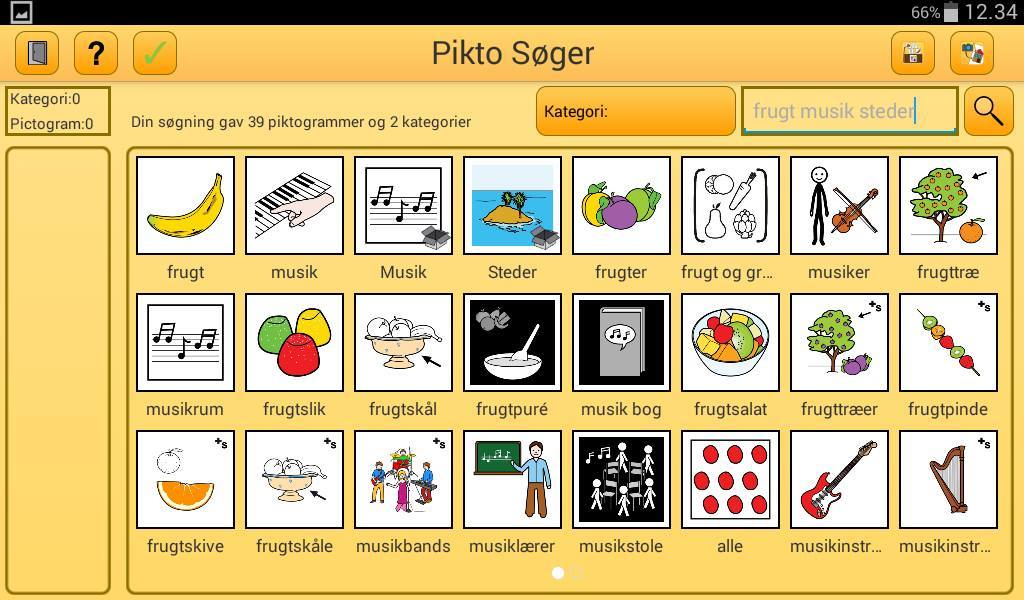
\includegraphics[width=0.75\textwidth]{sprint_three/pictosearch_view_pager}
    \caption{\ps with \androidinline{ViewPager}}
    \label{fig:pictosearch_view_pager}
\end{figure}

\FloatBarrier
This solution was later found to be inconsistent with other projects, in regards to the method of displaying pictograms. It was therefore decided that there should be a distinction between how applications and pictograms should be presented. For this reason, we assisted \emph{SW613F15} with implementing a \androidinline{GridView}, just like the one implemented in the \ct. The final result of \ps can be seen in \figref{fig:pictosearch}.

\begin{figure}[!htbp]
    \centering
    \includegraphics[width=0.75\textwidth]{sprint_three/pictosearch}
    \caption{Resulting application look for \ps}
    \label{fig:pictosearch}
\end{figure}